Computational geometry studies data structures and algorithms
useful to describe and solve geometrical problems. It goes from
computing basic geometrical magnitudes (distances, angles)
to the construction of efficient representations of geometrical
data for fast queries (e.g. nearest neighbours to a given point in space),
to the computation of geometrical relations between objects in
a metric space (visibility, connectivity, reachability).

In this chapter we will study a few basic geometrical problems,
and their computational solution, based on the tools available
on \sct. The \code{Geometry} namespace contains most of the 
geometry-related algorithms implemented in \sct. However, geometrically
related data structures, such as kd-trees and r-trees are found
under the \code{Collections} namespace instead.

\section{Convex Hull}\label{sec:convex-hull}

A
\cuttothechase{algorithm:graham-scan}{Graham's Scan}
\cuttothechase{algorithm:jarvis-march}{Jarvis March}
classic problem in computational geometry is the construction
of the convex hull of a set of points. Informally, the convex
hull is the minimum area convex polygon (in $R^2$) that surrounds the given set of points.
Extensions to $R^3$ and beyond are possible but considerably more complicated
than for $2$ dimensions.
If no three points are collinear, the convex hull
can be shown to be unique. In the other case, we can consider
to include or not the middle point(s), since the convex hull
area will remain the same. For simplicity, we will most of the time consider
this restriction to hold, since points with real coordinates
have a very small (probabilistically zero) chance of being collinear. 
However, the algorithms presented in this
section are oblivious to this restriction, and will simply drop (or not)
the middle point(s).

\begin{figure}
 \begin{center}
  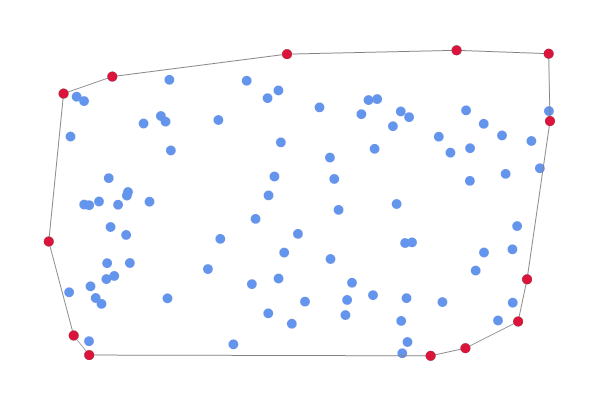
\includegraphics[width=0.8\textwidth]{Graphics/ConvexHullExample}
 \end{center}
 \caption[Convex Hull Example]{An example of the convex hull of a set of points in $R^2$.}
\end{figure}

Convex hulls seem to have no immediate application to real life problems.
However, they appear in the solution to many problems in 
CAD\footnote{Computer Aided Design} and computer simulation.

\subsection{Properties of Convex Hulls}\label{sub:convex-hull-properties}

Before diving into the algorithms we will discuss some basic 
properties of convex hulls, which allow us to build efficient
techniques to build them. 

First of all, there are a few points that will necessary be in the
convex hull. These are the \emph{extremal} points. The topmost,
leftmost, rightmost and bottommost points can be seen to fall
in this category easily. Note that some of these points can coincide.
For instance, the leftmost can also be the topmost or bottommost point.
For this reason, it is always safe to start building the convex at
one of these points. Again, if you have a tie, lets say, two points
with the minimum $x$, you'll need to break ties by choosing the 
upper (or lower) one. If both points also have the same $y$ then
they are the same point!

Since convex hulls are, well, convex, we can easily prove that
when walked in clockwise (or counter-clockwise) order, all points
turn to the same side. This will be the basic property used
by the Graham's scan algorithm (see the section \ref{sub:graham-scan}).
We can also prove that for every pair of adjacent points $x_i$, $x_{i+1}$ in the convex
hull (when taken clock-wise) the angle of the segment $\overline{x_i\,x_{i+1}}$
with respect to the horizontal (or any other reference line)
must be greater or equal than the angle
$\overline{x_i\,x_j}$ for any other $x_j$.
Otherwise the point $x_j$ would be outside the convex hull. This
property is key to prove to correctness of the Jarvis march algorithm
(see section \ref{sub:jarvis-march}).

\subsection{Graham's Scan}\label{sub:graham-scan}

\subsubsection*{Using Graham's Scan in \sct}\label{algorithm:graham-scan}

\subsection{Jarvis' March}\label{sub:jarvis-march}

\subsubsection*{Using Graham's Scan in \sct}\label{algorithm:graham-scan}